\chapter{Конструкторская часть}

В этом разделе будут представлены требования к программному обес-
печению (ПО), трудоемкость и схема алгоритмов.

\section{Требования к программному обеспечению}

Программе передаются массив целыми числами и элемент, который необходимо найти, а на выход получается индекс элемента массива. Кроме того, необходимо сообщить пользователю затраченное каждым алгоритмом процессорное время.

В создаваемом приложении пользователю должен быть доступен выбор желаемого алгоритма.

\section{Разработка стандартного алгоритма поиска}

На рисунке~\ref{fig:standart} представлен стандартный алгоритм поиска.

\begin{figure}[h!]
	\centering{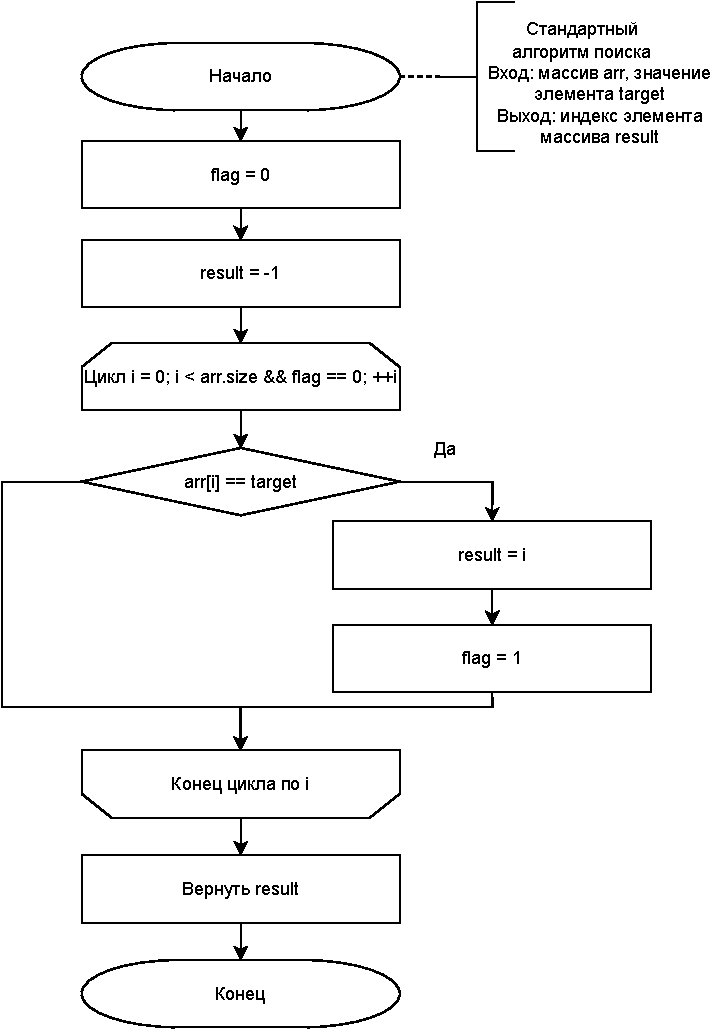
\includegraphics[scale=0.9]{photos/standart_search.pdf}}
	\caption{Стандартный алгоритм поиска}
	\label{fig:standart}
\end{figure}

\clearpage

\section{Разработка алгоритма бинарного поиска}

На рисунке~\ref{fig:binary} представлен алгоритм бинарного поиска.

\begin{figure}[h!]
	\centering{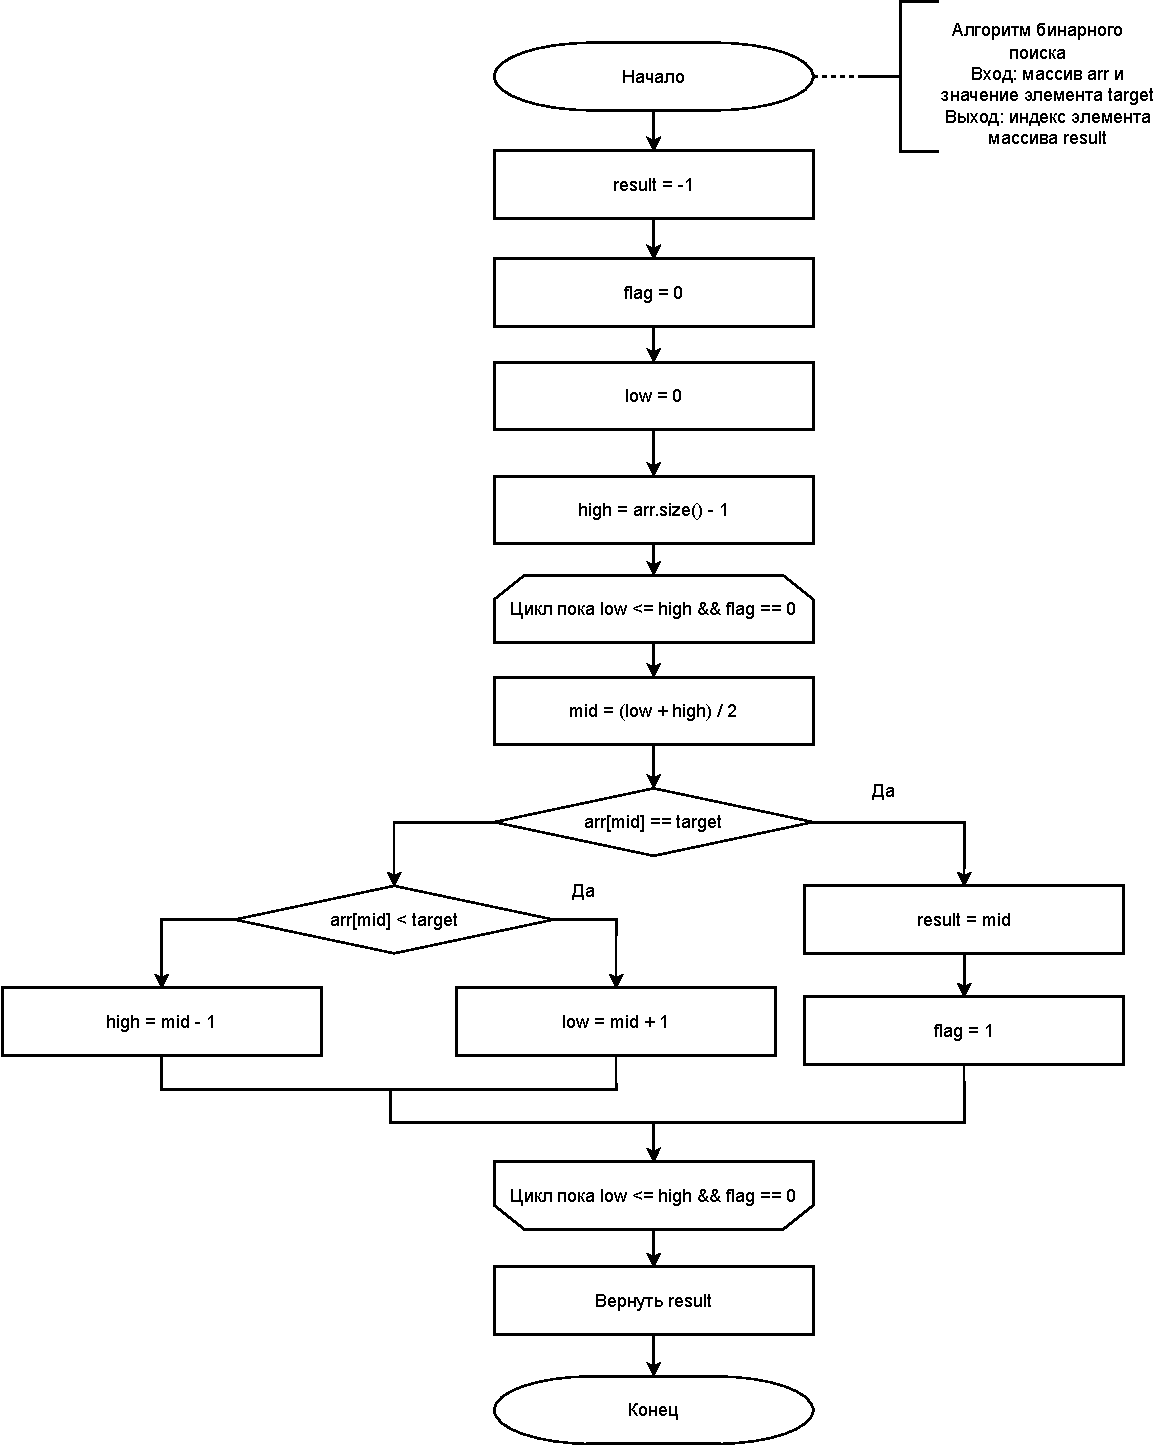
\includegraphics[scale=0.65]{photos/binary_search.pdf}}
	\caption{Алгоритм бинарного поиска}
	\label{fig:binary}
\end{figure}

\section{Модель вычислений}

Для дальнейшего анализа трудоемкости необходимо ввести модель вычислений.

Операции из списка (\ref{for:opers}) имеют трудоемкость 1.

\begin{equation}
	\label{for:opers}
	=, +=, -=, +, -, ==, !=, <, >, <=, >=, [], ++, {-}-
\end{equation}

Операции из списка (\ref{for:opers2}) имеют трудоемкость 2.

\begin{equation}
	\label{for:opers2}
	*, /, \%
\end{equation}

Трудоемкость оператора выбора \code{if условие then A else B} рассчитывается как:

\begin{equation}
	\label{for:if}
	f_{if} = f_{\text{условия}} +
	\begin{cases}
		f_A, & \text{если условие выполняется,}\\
		f_B, & \text{иначе.}
	\end{cases}
\end{equation}

Трудоемкость цикла рассчитывается как:

\begin{equation}
	\label{for:for}
	f_{for} = f_{\text{инициализации}} + f_{\text{сравнения}} + N(f_{\text{тела}} + f_{\text{инкремента}} + f_{\text{сравнения}})
\end{equation}

Трудоемкость вызова функции равна 0.

\section{Трудоемкость алгоритмов}

Далее размер массива обозначается как $N$.

\subsection{Стандартный алгоритм поиска}

Пусть на старте алгоритм затрагивает $k_0$ операций, а при сравнении $k_1$ операций, тогда:

\begin{itemize}
	\item в лучшем случае элемент будет найден на первом сравнении за $k_0 + k_1$ операций;
	\item в худшем случае элемент будет найден на последнем сравнении за $k_0 + N · k_1$ операций;
	\item элемент будет найден на i-ом сравнении за $k_0 + i · k_1$ операций.
\end{itemize}

Тогда средняя трудоемкость может быть рассчитана по следующей формуле:

\begin{equation}
	f = k_0 + k_1 \cdot \left(1 + \frac{N}{2} - \frac{1}{N + 1}\right)
\end{equation}

\subsection{Алгоритм бинарного поиска}

Пусть на старте алгоритм затрагивает $k_0$ операций, тогда: 

\begin{itemize}
	\item в лучшем случае элемент будет найден на первом сравнении с средним элементом с трудоемкостью $k_0$ + $log_2 1$;
	\item в худшем случае элемент будет найден на последнем сравнении с трудоёмкостью $b + log_2 N$;
	\item элемент будет найден на i-ом сравнении с трудоемкостью $b + log_2 i$;
\end{itemize}

\section*{Вывод}

На основе теоретических знаний, полученных в аналитическом разделе, были разработаны схемы алгоритмов, благодаря которым может быть найден элемент массива разными способами. 
Также для каждого из них были рассчитаны и оценены лучшие и худшие случаи.
